\documentclass[9pt, aspectratio=169]{beamer}
\usepackage{FiraSans}
\usetheme[subsectionpage=progressbar]{metropolis}
\usepackage[utf8]{inputenc}
\usepackage{amsmath}
\usepackage{amsfonts}
\usepackage{amssymb}
\usepackage{multicol}
\usepackage{tikz}
\usepackage{caption}
\usepackage{xcolor}
\usepackage[T1]{fontenc} 
\usepackage[skins]{tcolorbox}
\author{Nicola Roman\`o - nicola.romano@ed.ac.uk}
\title{Lecture 19 - Recents advances in image analysis using deep learning\\\small Part 1 - Image improvement}
\setlength{\fboxsep}{0pt}
\setbeamertemplate {footline}{\begin{scriptsize}\hfill\insertframenumber ~of \inserttotalframenumber\kern1em\vskip5pt\end{scriptsize}}

% Remove "Figure" in front of captions
% See https://tex.stackexchange.com/questions/82456/how-to-remove-figure-caption-prefix-figure-in-beamer
\captionsetup{labelformat=empty,labelsep=none}

\titlegraphic{\centering 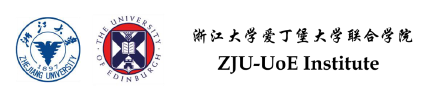
\includegraphics[scale=.5]{instituteLogo.png}}
\date{}

\begin{document}

\newtcolorbox{codebox}{enhanced,
    top=2pt,
    left=2pt,
    right=2pt,
    bottom=2pt,
    boxrule=0pt,
    leftrule=5pt,
    sharp corners,
    colback=gray!20,
    colframe=blue!60!black}

\begin{frame}
    \titlepage
\end{frame}

\begin{frame}
    {Learning objectives}
    \begin{columns}
        \begin{column}{0.8\textwidth}
            \begin{itemize}
                \item Discuss recent advances in image analysis using deep learning.
            \end{itemize}

            \pause
            \vspace{2em}

            Today we are going to analyse recent articles related to image improvement using deep learning.

            \begin{itemize}
                \item Noise removal
                      \begin{itemize}
                          \item Lehtinen et al. 2018 - Noise2Noise: Learning Image Restoration without Clean Data
                          \item Krull et al. 2019 - Noise2Void: Learning Denoising from Single Noisy Images
                      \end{itemize}
                \item Superresolution
                      \begin{itemize}
                          \item Wang et al. 2019 - Deep learning enables cross-modality
                                super-resolution in fluorescence microscopy
                      \end{itemize}
                \item Refocusing
                      \begin{itemize}
                          \item Wu et al. 2019 - Three-dimensional virtual refocusing of fluorescence microscopy images using deep learning
                      \end{itemize}
            \end{itemize}
        \end{column}
        \begin{column}{0.2\textwidth}
            
\includegraphics[angle=-30, origin=tr, width=1.5\textwidth]{lightbulb.png}
        \end{column}
    \end{columns}
\end{frame}

\section{Noise removal}

\begin{frame}
    {The problem}
    \begin{itemize}
        \item Noise is a major problem in image analysis and very common in biomedical imaging.
        \item Image denoising tries to separate the image signal from noise. Existing methods rely on the assumptions that pixel values in the noise component are uncorrelated.
        \item CNN can be used to remove noise from images by training them on pairs of noisy and clean images.
        \item Often we don't have access to clean images.
        \item Can we just train on noisy images?
    \end{itemize}
\end{frame}

\begin{frame}
    {Noise2Noise}
    \centering
    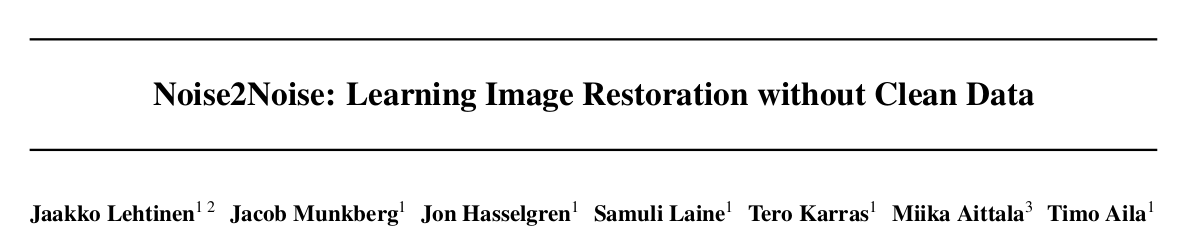
\includegraphics[width=\textwidth]{Noise2Noise_title.png}
\end{frame}

\begin{frame}
    {Noise2Noise - architecture}
    \centering
    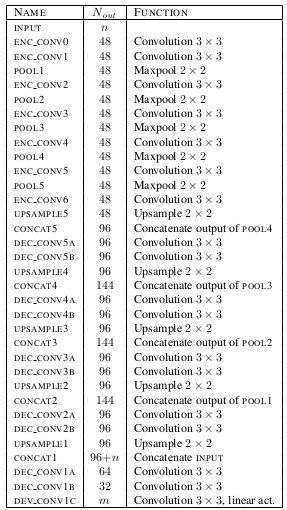
\includegraphics[width=.3\textwidth]{noise2noise_architecture.png}
\end{frame}

\begin{frame}
    {Noise2Noise - results}
    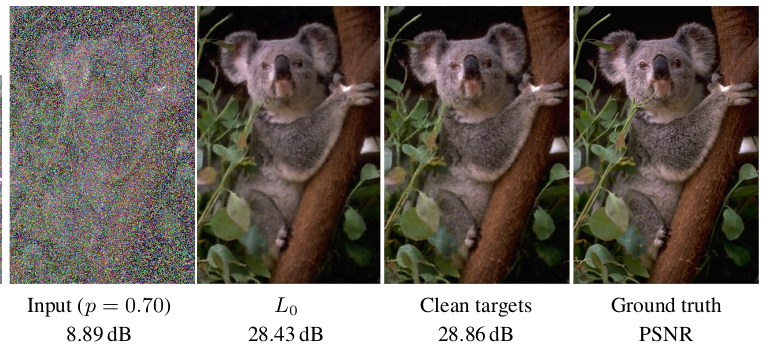
\includegraphics[width=\textwidth]{noise2noise_results.png}
\end{frame}

\begin{frame}
    {Beyond Noise2Noise - Noise2Void}
    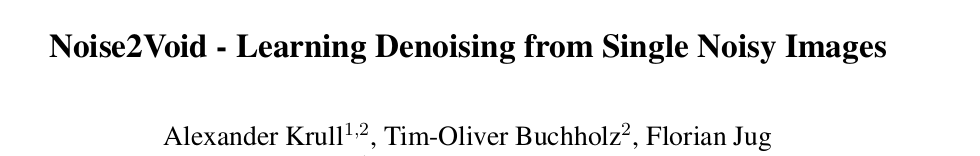
\includegraphics[width=\textwidth]{Noise2Void_title.png}
\end{frame}

\begin{frame}
    {Noise2Void - the process}
    \centering
    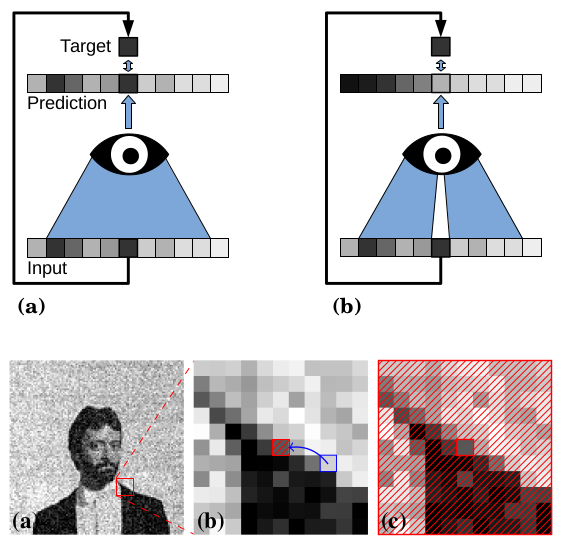
\includegraphics[width=.5\textwidth]{Noise2Void_process.png}
\end{frame}
\begin{frame}
    {Noise2Void - results}
    \centering
    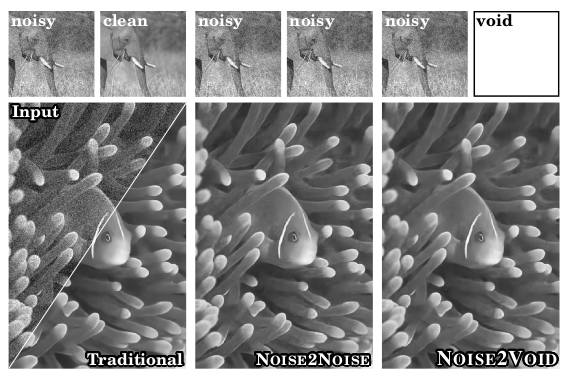
\includegraphics[width=.8\textwidth]{Noise2Void_result.png}
\end{frame}

\begin{frame}
    {Comparison of denoising methods}
    \centering\ 1
    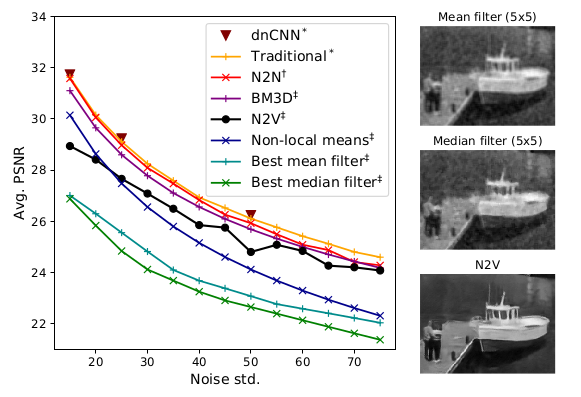
\includegraphics[width=.7\textwidth]{denoising comparison.png}
\end{frame}
\section{Refocusing}

\begin{frame}
    {The problem}
    \begin{itemize}[<+->]
        \item Volumetric fluorescence is widely used in many biological imaging applications.
        \item Acquired e.g. using confocal, two photon or light sheet microscopy.
        \item Problems include speed, phototoxicity, photobleaching.
        \item Widefield microscopy is much faster but has lower resolution and loses the volumetric information.
    \end{itemize}

    \only<2>
    {
        \centering
        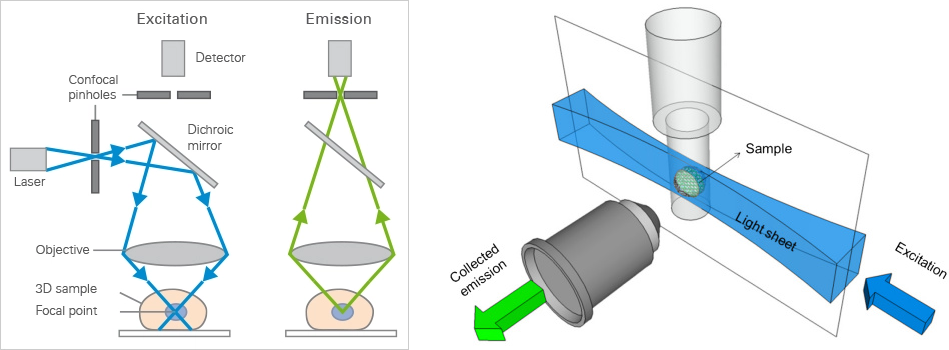
\includegraphics[width=.8\textwidth]{confocal_lightsheet.png}
    }
    \only<4>
    {
        \centering
        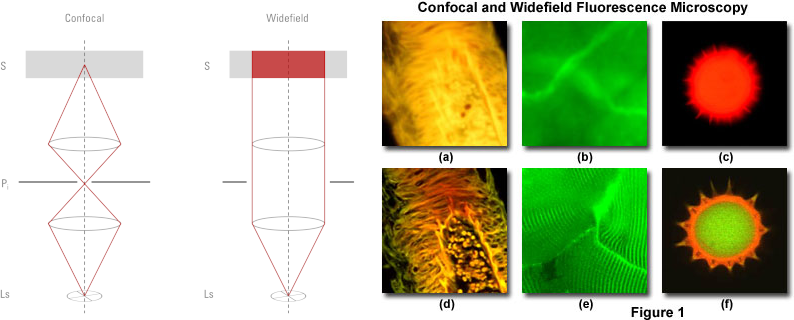
\includegraphics[width=.8\textwidth]{Confocal_vs_Widefield.png}
    }
\end{frame}

\begin{frame}
    {Deep-Z}
    Can we refocus using deep learning?
    Can we use widefield microscopy images to reconstruct the lost volumetric information?

    \centering
    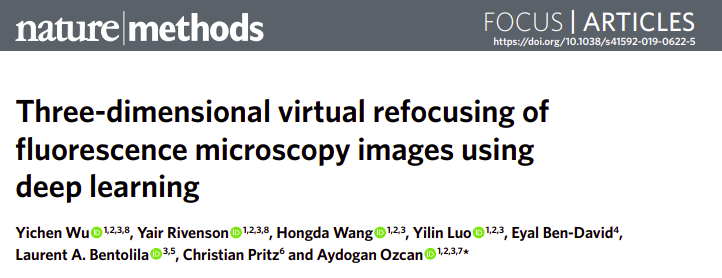
\includegraphics[width=.8\textwidth]{wu_2019_title.png}

    \pause
    \raggedright
    ``Here we introduce a digital image refocusing framework in fluorescence microscopy by training a deep neural network using microscopic image data, enabling 3D imaging of fluorescent samples using a single 2D wide-field image, without the need for any
    mechanical scanning, additional hardware or parameter estimation.''
\end{frame}

\begin{frame}
    {How does it work?}
    \begin{itemize}[<+->]
        \item Given a widefield image, Deep-Z associates to it a user-defined \textit{digital propagation matrix} (DPM) containing the desired axial distance of the target surface from the plane of the input image.
        \item Deep-Z uses a generative-adversarial network (GAN) to generate synthetic images that approximates the desired depth.
        \item It is trained on ``matched pairs of (1) various fluorescence images axially focused at different depths and appended with different DPMs, and (2) the corresponding fluorescence images (that is, the ground-truth labels) captured at the correct (target) focus plane defined by the corresponding DPM.''
    \end{itemize}
\end{frame}

\begin{frame}
    {Deep-Z - the process}
    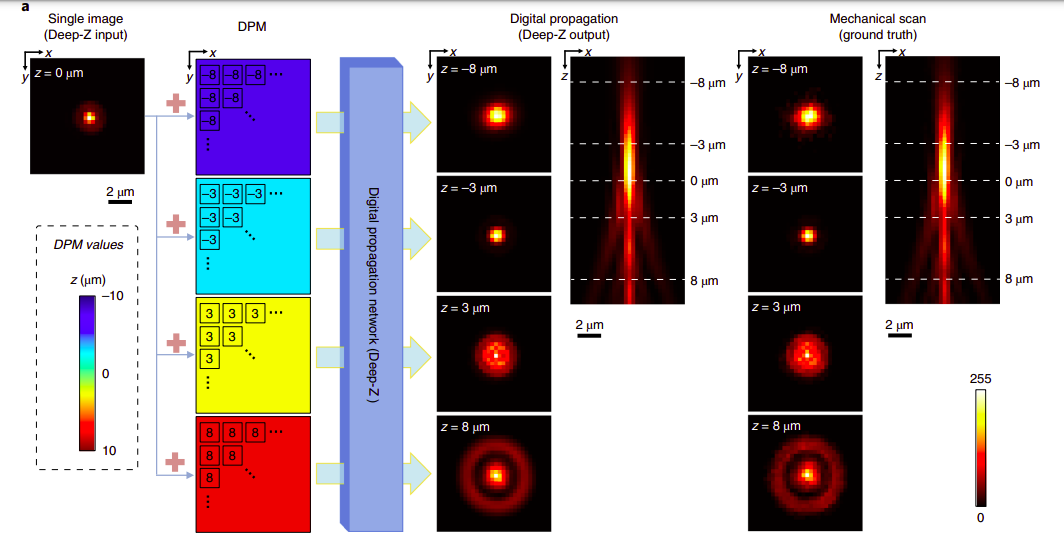
\includegraphics[width=\textwidth]{deepz_process.png}
\end{frame}
\begin{frame}
    {Generative-adversarial-networks (GANs)}
    \textbf{GANs} are a class of neural networks that are able to learn to generate new images from a training set of images.

    \pause
    They consist of two parts:
    \begin{itemize}
        \item The \textbf{generator}, a neural network that generates new images.
        \item The \textbf{discriminator}, a neural network that determines whether an image is real or generated.
    \end{itemize}

    \pause
    The generator and the discriminator \textit{fight} each other (hence the network is \textit{adversarial}), so the generator has to improve in order to be able to \textit{fool} the discriminator into thinking its images are real.
\end{frame}

\begin{frame}
    {GAN - simplified schematic}
    \centering
    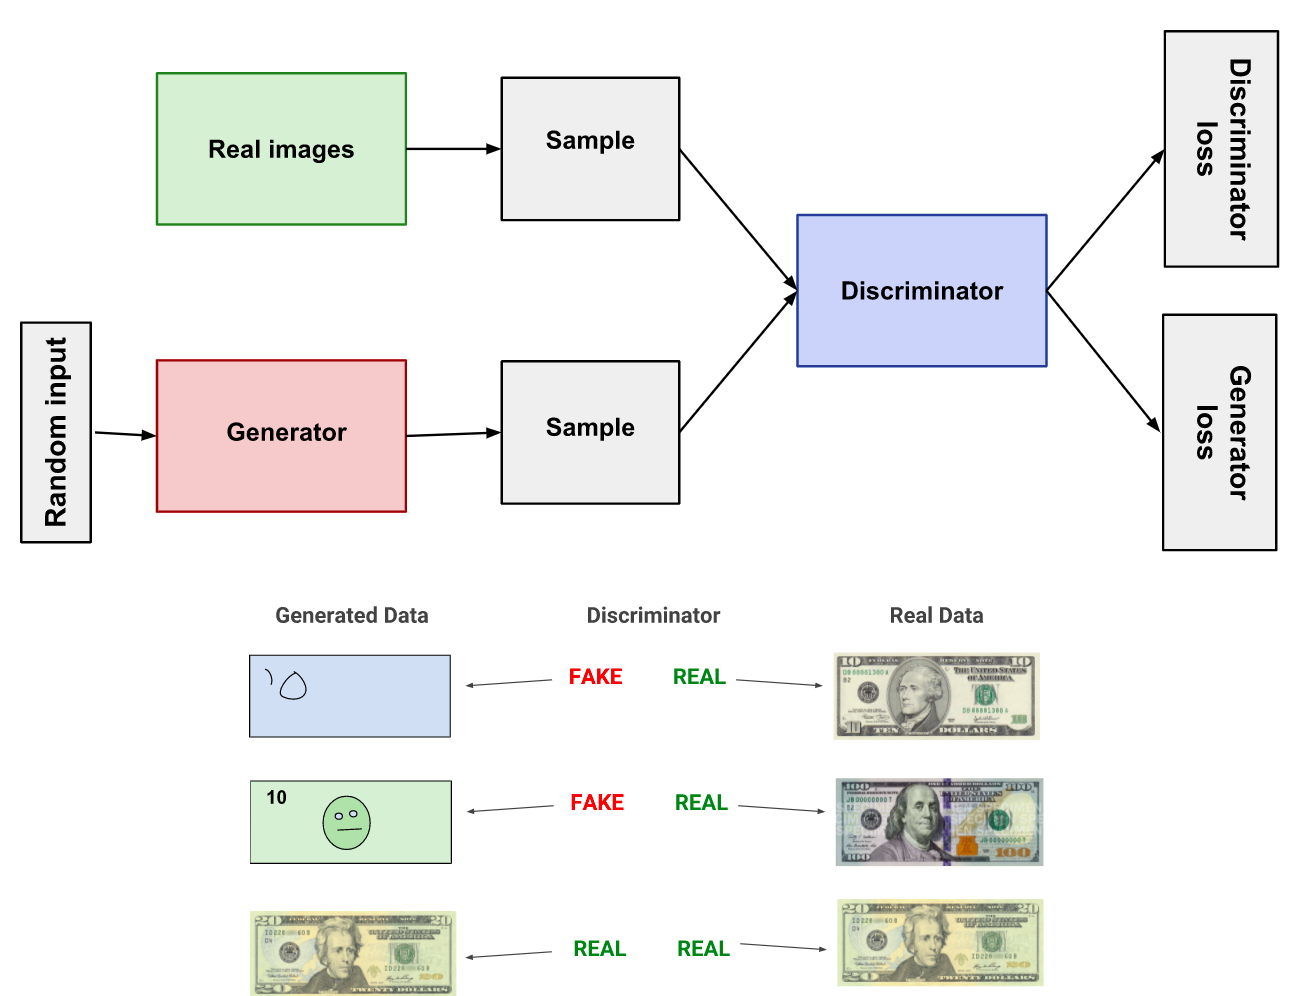
\includegraphics[width=.65\textwidth]{GAN.png}

    \footnotesize
    \raggedright
    Source: Google Developers
\end{frame}

\begin{frame}
    {Deep-Z - results}
    \centering
    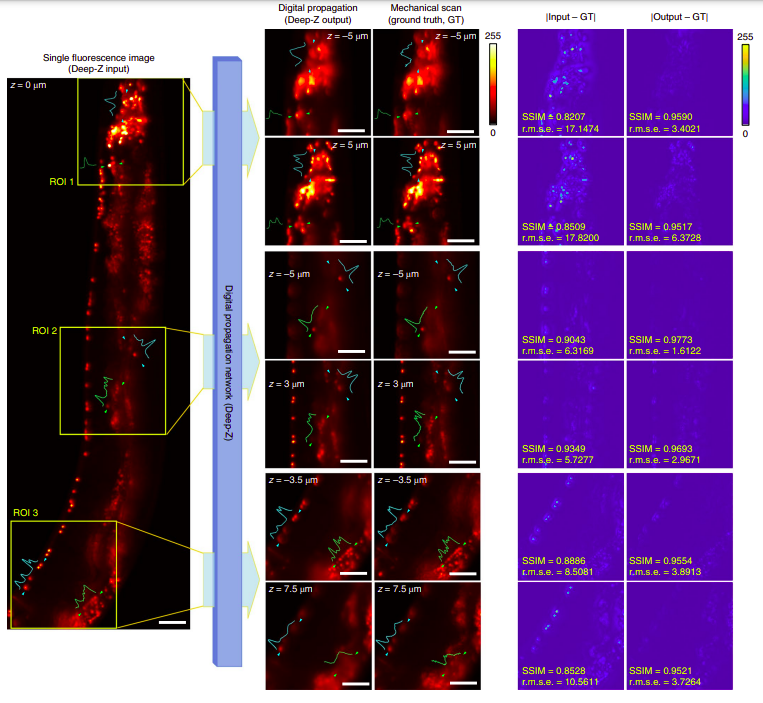
\includegraphics[width=.6\textwidth]{deepz_results.png}
\end{frame}

\begin{frame}
    {Non-uniform DPMs}
    \only<1>
    {
        \centering
        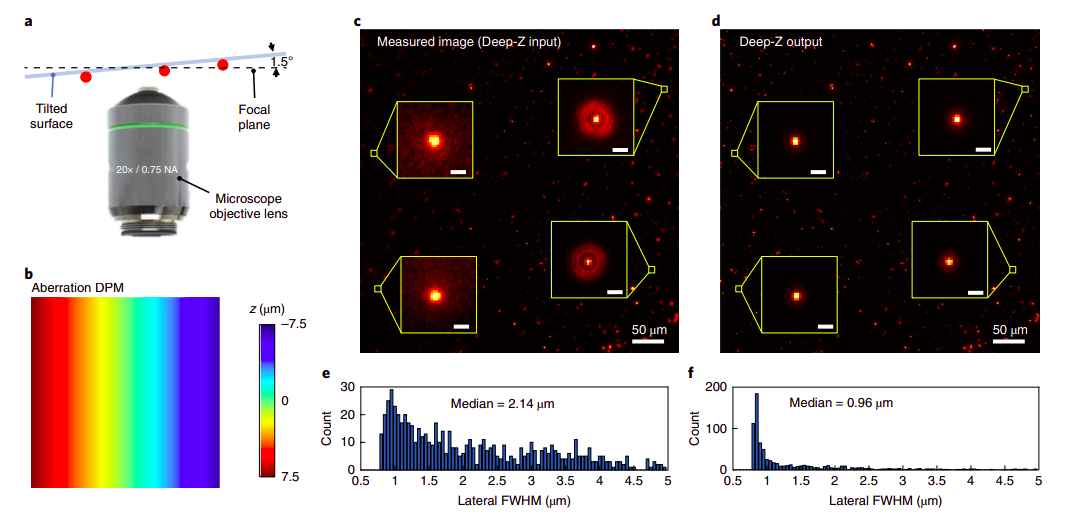
\includegraphics[width=.8\textwidth]{tilted_DPM.png}
    }
    \only<2>
    {
        \centering
        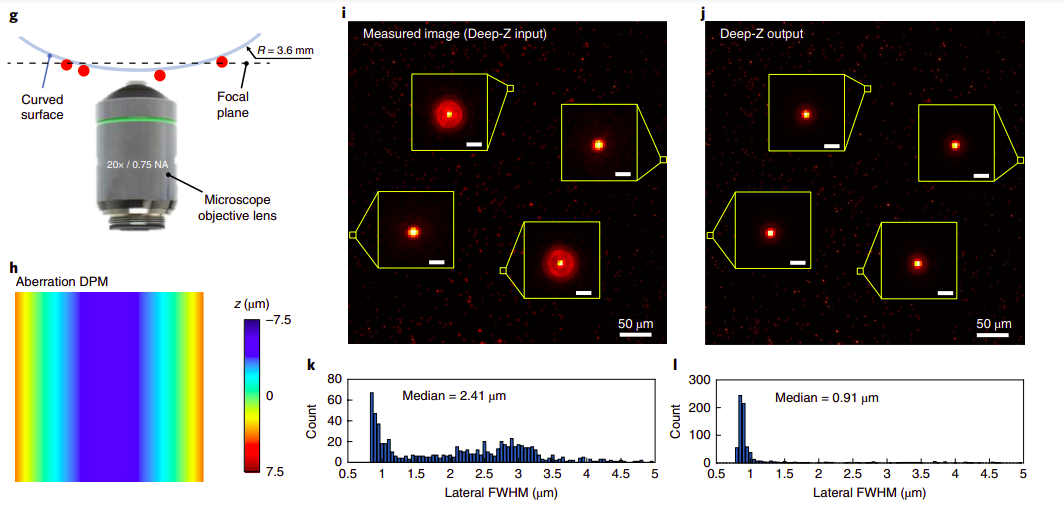
\includegraphics[width=.8\textwidth]{curved_DPM.png}
    }
\end{frame}

\begin{frame}
    {Deep-Z+ - cross-modality refocusing}
    Deep-Z+ allows cross-modality refocusing.

    \centering
    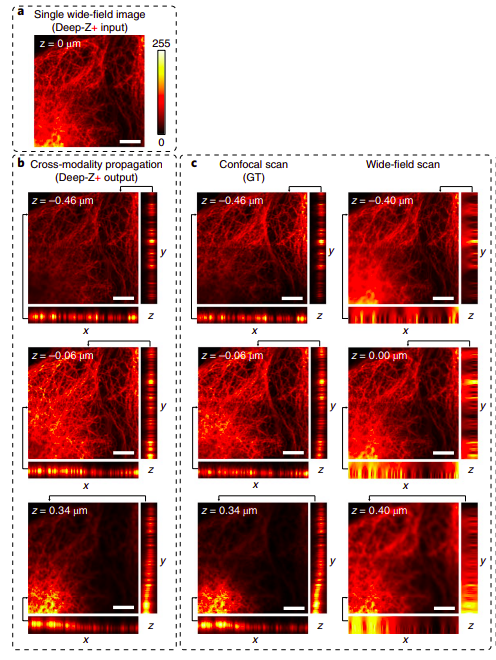
\includegraphics[width=.4\textwidth]{deepzplus.png}
\end{frame}

\section{Superresolution}

\begin{frame}
    {The problem}
    \begin{itemize}
        \item Super-resolution methods such as STED or SIM allow the study of biological processes at a finer resolution than the resolution of the microscope.
        \item They require expensive setups, specific sample preparation and extensive post-processing.
        \item Post-processing requires \textit{a priori} knowledge of the sample/mounting media/imaging system etc.
    \end{itemize}
\end{frame}
\begin{frame}
    {Deep learning for superresolution}
    \centering
    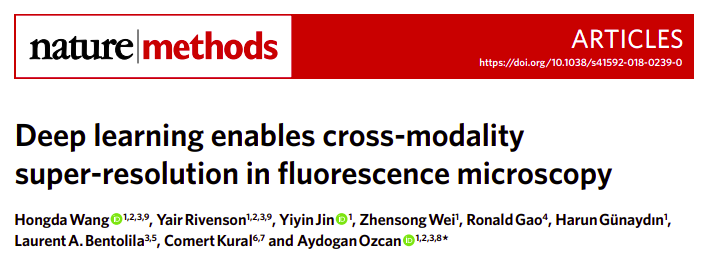
\includegraphics[width=\textwidth]{wang_title.png}

    ``Here we present a deep-learning-based framework to achieve super-resolution and cross-modality image transformations in fluorescence microscopy without the need for making any assumptions about or modeling of the image-formation process.''
\end{frame}

\begin{frame}
    {The process}
    ``We trained a deep neural network using a generative adversarial network (GAN)16 model to transform an acquired low-resolution image into a high-resolution one using matched pairs of experimentally acquired low- and  higher-resolution images. [\dots] Once the deep network is trained, it remains fixed and can be used to rapidly output batches of high-resolution images in, for
    example, 0.4 s for an image size of 1,024$\times$1,024 pixels using a single graphics processing unit (GPU).
\end{frame}

\begin{frame}
    {The results}
    \centering

    \only<1>
    {
        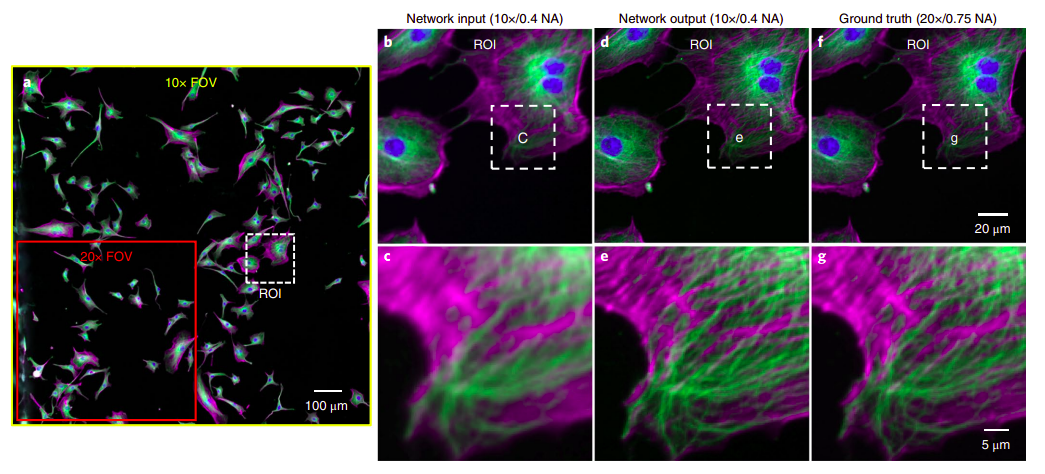
\includegraphics[width=.8\textwidth]{wang_results.png}

        \footnotesize
        \raggedright
        Deep-learning-based super-resolved images of bovine pulmonary artery endothelial cells.Color map: magenta for F-actin, green for microtubules, blue for nuclei.
    }
    \only<2>
    {
    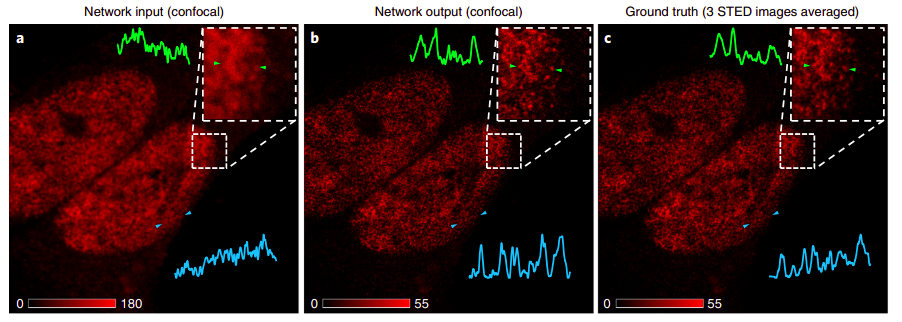
\includegraphics[width=.8\textwidth]{confocal2sted.png}

    \footnotesize
    \raggedright
    Cross-modality transformation from confocal to STED.
    }
\end{frame}
\end{document}